\documentclass[]{beamer}

\usepackage{fontspec} 
% \usepackage{lsp-makros}
\useoutertheme{lsp}

\usepackage{lsptitle}

\def\two@digits#1{\ifnum#1<10 0\fi\number#1}
\def\mytoday{\two@digits{\number\day}.\two@digits{\number\month}.\number\year}


\usepackage{xspace,multicol}
\newcommand{\latex}{\LaTeX\xspace}
\usepackage{tikz}


\newcounter{lastpagemainpart}
\footnotesep0pt
\renewcommand{\footnoterule}{}
\usefootnotetemplate{
  \noindent
  \insertfootnotemark\insertfootnotetext}

\let\beamerfn=\footnote
\renewcommand{\footnote}[1]{%
\let\oldfnsize=\footnotesize%
\let\footnotesize=\tiny%
\beamerfn<\thebeamerpauses->{#1}%
\let\footnotesize=\oldfnsize}


\date{\today}

\usepackage{eurosym}  
 
\renewcommand{\centerline}[1]{\hfill#1\hfill\hfill\mbox{}}
\newcommand{\highlight}{\mdseries\color{red!80!black}}

\title{Accès libre -- Open Access\\For whom -- pour qui?}
% \institute{FU Berlin}
\author[Nordhoff]{Sebastian Nordhoff}
\date{FieldLing, Paris, 2021-09-10}


\begin{document}
\lspbeamertitle

\section{Introduction}

\frame{
\frametitle{Outline}
\tableofcontents
}

\frame{
\frametitle{Sebastian Nordhoff}
%   \includegraphics[height=.2\textheight]{./path/to/graphicsfile}
  \begin{itemize}
    \item PhD 2009 \textit{A grammar of Upcountry Sri Lanka Malay}
    \item 3 edited volumes, about 30 research articles
    \item 2009-2012 Glottolog.org at the Max Planck Institute for Evolutionary Anthropology
    \item advocate for Open Source, Open Access, Open Data, Open Everything 
    \item since 2014 coordinator for Language Science Press
    \item involved in the publication of 150+ books since 2014
  \end{itemize}
}

\frame{
\frametitle{Language Science Press}
%   \includegraphics[height=.2\textheight]{./path/to/graphicsfile}
  \begin{itemize}
    \item  scholar-owned, community-based publisher 
    \item Open Access
    \item free to read 
    \item free to publish 
    \item 29 series
    \item 30 books a year (monographs and edited volumes)
    \item Publisher for both the Pāṇini award (Grimm, Nadine. 2021. \textit{A Grammar of Gyeli}) and the Greenberg award winners of the Association for Linguistic Typology (Easterday, Shelece. 2020. \textit{Highly complex syllable structure})
    \end{itemize}
}

\frame{
\frametitle{Language Science Press}
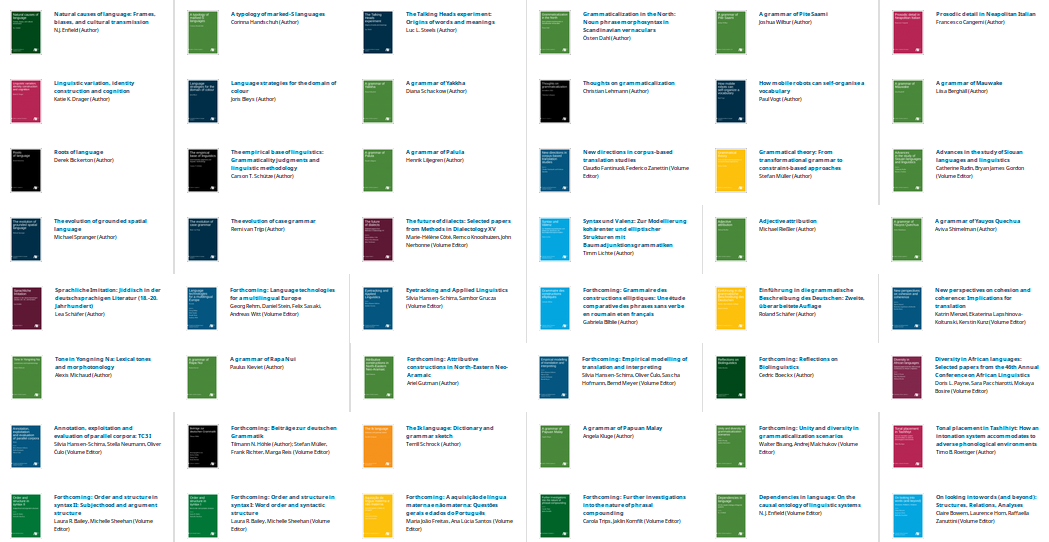
\includegraphics[height=\textheight]{catalog.png}
}
% 
% \frame{
% \frametitle{Production of a book:\\ traditional model}
% %   \includegraphics[height=.2\textheight]{./path/to/graphicsfile}
%   \begin{enumerate}
%     \item inquiry
% 	\item book proposal
% 	\item proposal approval
% 	\item contract
% 	\item first submission
% 	\item review
% 	\item first decision
% 	\item revision
% 	\item final decision
% 	\item copyediting
% 	\item first proofs
% 	\item typesetting
% 	\item final proofs
%   \end{enumerate}
% }


\frame{
\frametitle{Tenets}
%   \includegraphics[height=.2\textheight]{./path/to/graphicsfile}
  \begin{itemize}
\item    We want to share our knowledge
\item     We want to arrive at new findings regarding human language(s) and share these findings with everyone interested
\begin{itemize}
  \item         other researchers
  \item       speakers
  \item       general public
\end{itemize}
  \item   How can we achieve this goal?
 \end{itemize}
}

\frame{
\frametitle{The FAIR principles}
%   \includegraphics[height=.2\textheight]{./path/to/graphicsfile}
  \begin{itemize}
    \item  Findable
    \item Accessible
    \item Interoperable
    \item Reusable
  \end{itemize}
}

\frame{
\frametitle{Findable}
%   \includegraphics[height=.2\textheight]{./path/to/graphicsfile}
  \begin{itemize}
    \item  Use repositories
    \begin{itemize}
      \item do not use www.myname.com/thesis.pdf
      \item try to use domain specific repositories
    \end{itemize}
    \item Fill in all metadata fields as far as possible
    \begin{itemize}
      \item author name, title, subject, languages, coordinates
    \end{itemize}
  \end{itemize}
}

\frame{
\frametitle{Accessible}
  \begin{itemize}
    \item  no paywalls
    \item no complicated access protocols

  
\includegraphics[height=.2\textheight]{stefanmuellerpaywall.png}
  \end{itemize}
}

\frame{
\frametitle{Interoperable}
%   \includegraphics[height=.2\textheight]{./path/to/graphicsfile}
  \begin{itemize}
    \item  file formats should be
    \begin{itemize}
      \item standardised
      \item open
      \item well-suited for the purpose
    \end{itemize}
  \end{itemize}
}

\frame{
\frametitle{Interoperability}
   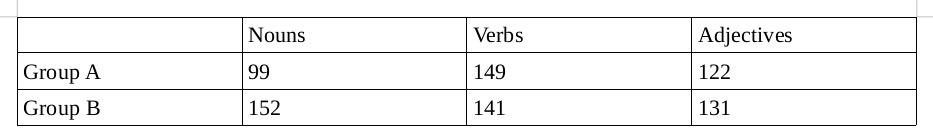
\includegraphics[height=.2\textheight]{sampletable_oo.png}
 }

\frame{
\frametitle{Interoperability PDF }
   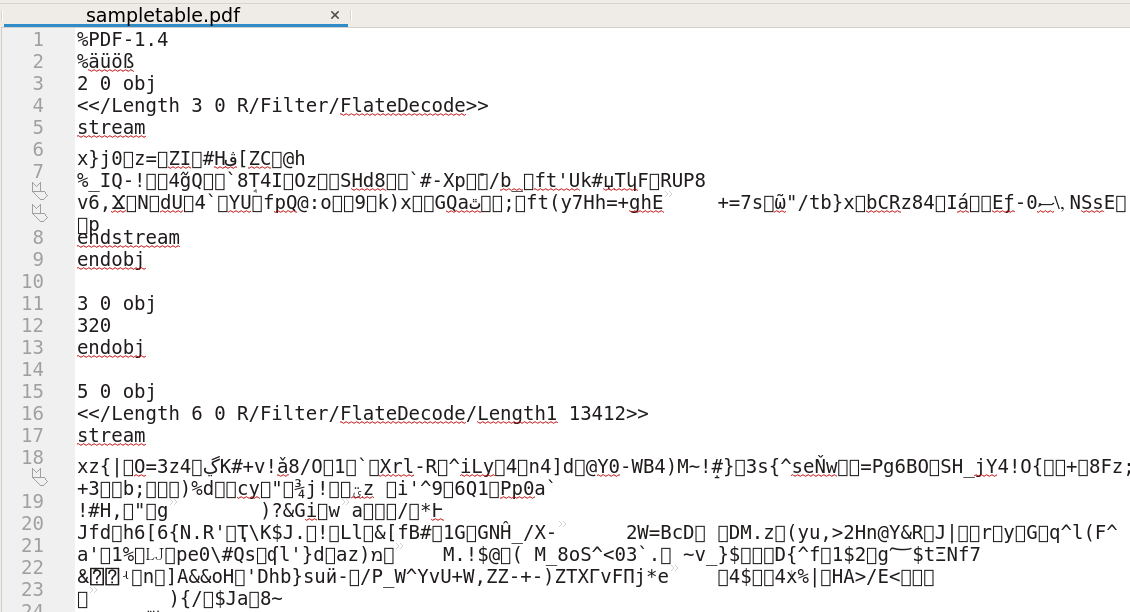
\includegraphics[height=.2\textheight]{sampletable_pdf.png}
 }

\frame{
\frametitle{Interoperability ODT/XML}
   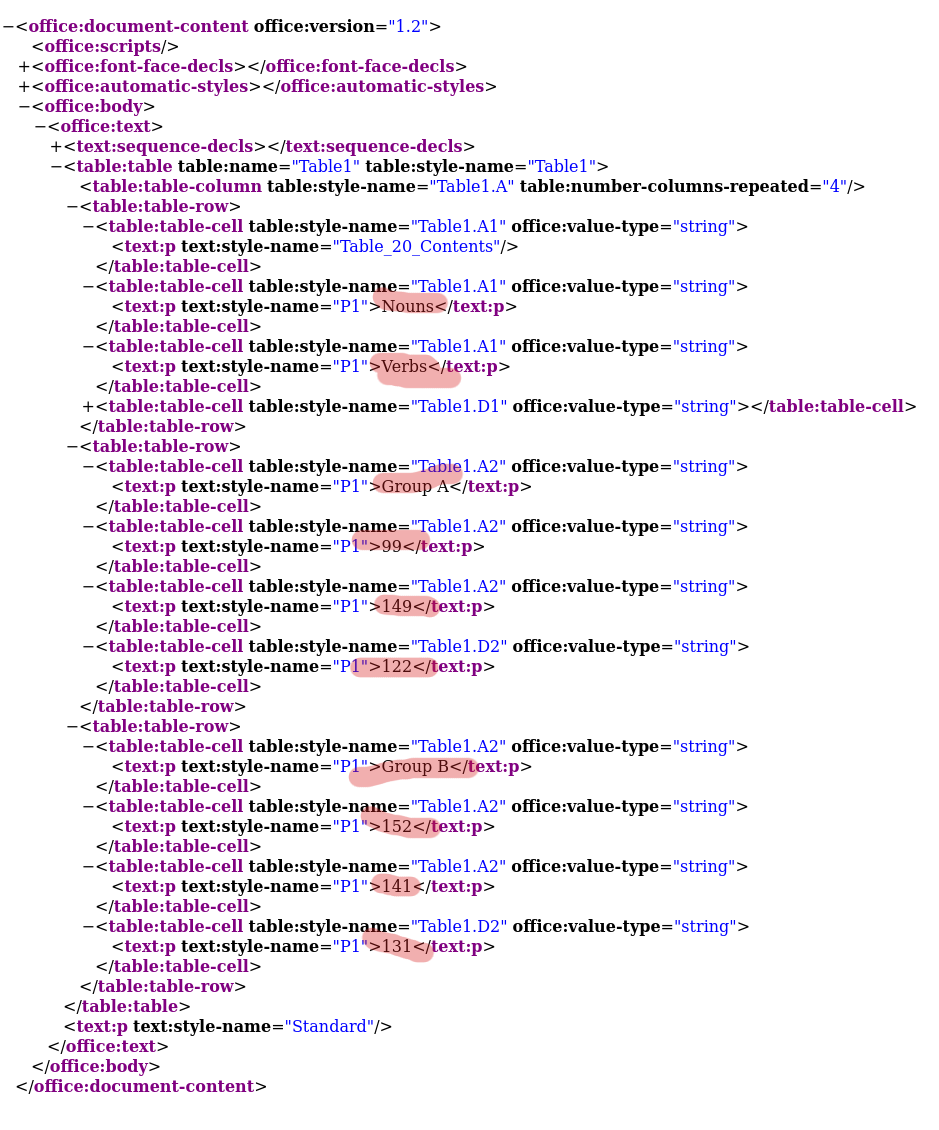
\includegraphics[height=.2\textheight]{sampletable_xml.png}
 }


\frame{
\frametitle{Interoperability CSV}
   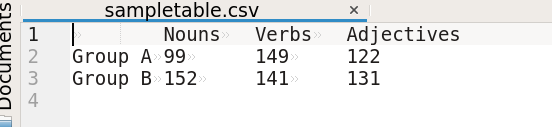
\includegraphics[height=.2\textheight]{sampletable_csv.png}
 }

 \frame{
\frametitle{Reusable}
%   \includegraphics[height=.2\textheight]{./path/to/graphicsfile}
  \begin{itemize}
    \item  who wants to reuse your data?
    \begin{itemize}
      \item unlikely: Disney, Walmart, Amazon
      \item likely: researchers, linguistic blog, language schools
    \end{itemize}
    \item choose a suitable license to allow reuse with attribution
  \end{itemize}
}

\frame{
\frametitle{Licenses}
%   \includegraphics[height=.2\textheight]{./path/to/graphicsfile}
  \begin{itemize}
    \item  Use a Creative Commons License
    \item good: CC-BY, CC-BY-SA
    \item bad: CC-BY-ND (no translations, no excerpts, no cropping, no recomposition)
    \item very bad: CC-BY-NC: no blogs with ads, no language schools, no exhibitions with fees.
    \item the worst: CC-BY-NC-ND
  \end{itemize}
}

 \frame{
\frametitle{The Bad Guys}
%   \includegraphics[height=.2\textheight]{./path/to/graphicsfile}
  \begin{itemize}
    \item Plagiarists and pirates
    \item Neither of them are stopped by (c) or restrictive licenses
    \item They know that what they do is illegal

  \end{itemize}
}

\frame{
\frametitle{Data, code, text}
%   \includegraphics[height=.2\textheight]{./path/to/graphicsfile}
  \begin{itemize}
    \item  Clearly separate your raw data, the code you use to analyze the data, and the write-up
    \item Different repositories exist for each
  \end{itemize}
}

\frame{
\frametitle{Frametitle3}
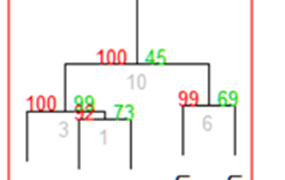
\includegraphics[width=\textwidth]{pngR2.png}
}

\frame{
\frametitle{Where to put your FAIR data? Repositories}
%   \includegraphics[height=.2\textheight]{./path/to/graphicsfile}
  \begin{itemize}
    \item Repositories collect documents and research data 
      \begin{itemize}
        \item \textbf{discipline-specific} or \textbf{general purpose}
        \item \textbf{preprint} or \textbf{postprint} 
        \item \textbf{text} or \textbf{data} or \textbf{code}
      \end{itemize}
  \end{itemize}
}

\frame{
\frametitle{Code repositories}
%   \includegraphics[height=.2\textheight]{./path/to/graphicsfile}
  \begin{itemize}
    \item  GitHub
    \item GitLab
  \end{itemize}
}

\frame{
\frametitle{Multimedia}
%   \includegraphics[height=.2\textheight]{./path/to/graphicsfile}
  \begin{itemize}
    \item  Paradisec
    \item ELAR
    \item AILLA
    \item TLA
  \end{itemize}
}

\frame{
\frametitle{Numerical data}
%   \includegraphics[height=.2\textheight]{./path/to/graphicsfile}
  \begin{itemize}
    \item TROLLing
    \item figshare
    \item GitHub/GitLab
    \item  Zenodo (also as a general fallback)
    \item GitHub-Zenodo bridge to integrate versioning and archiving
  \end{itemize}
}

\frame{
\frametitle{figshare}
   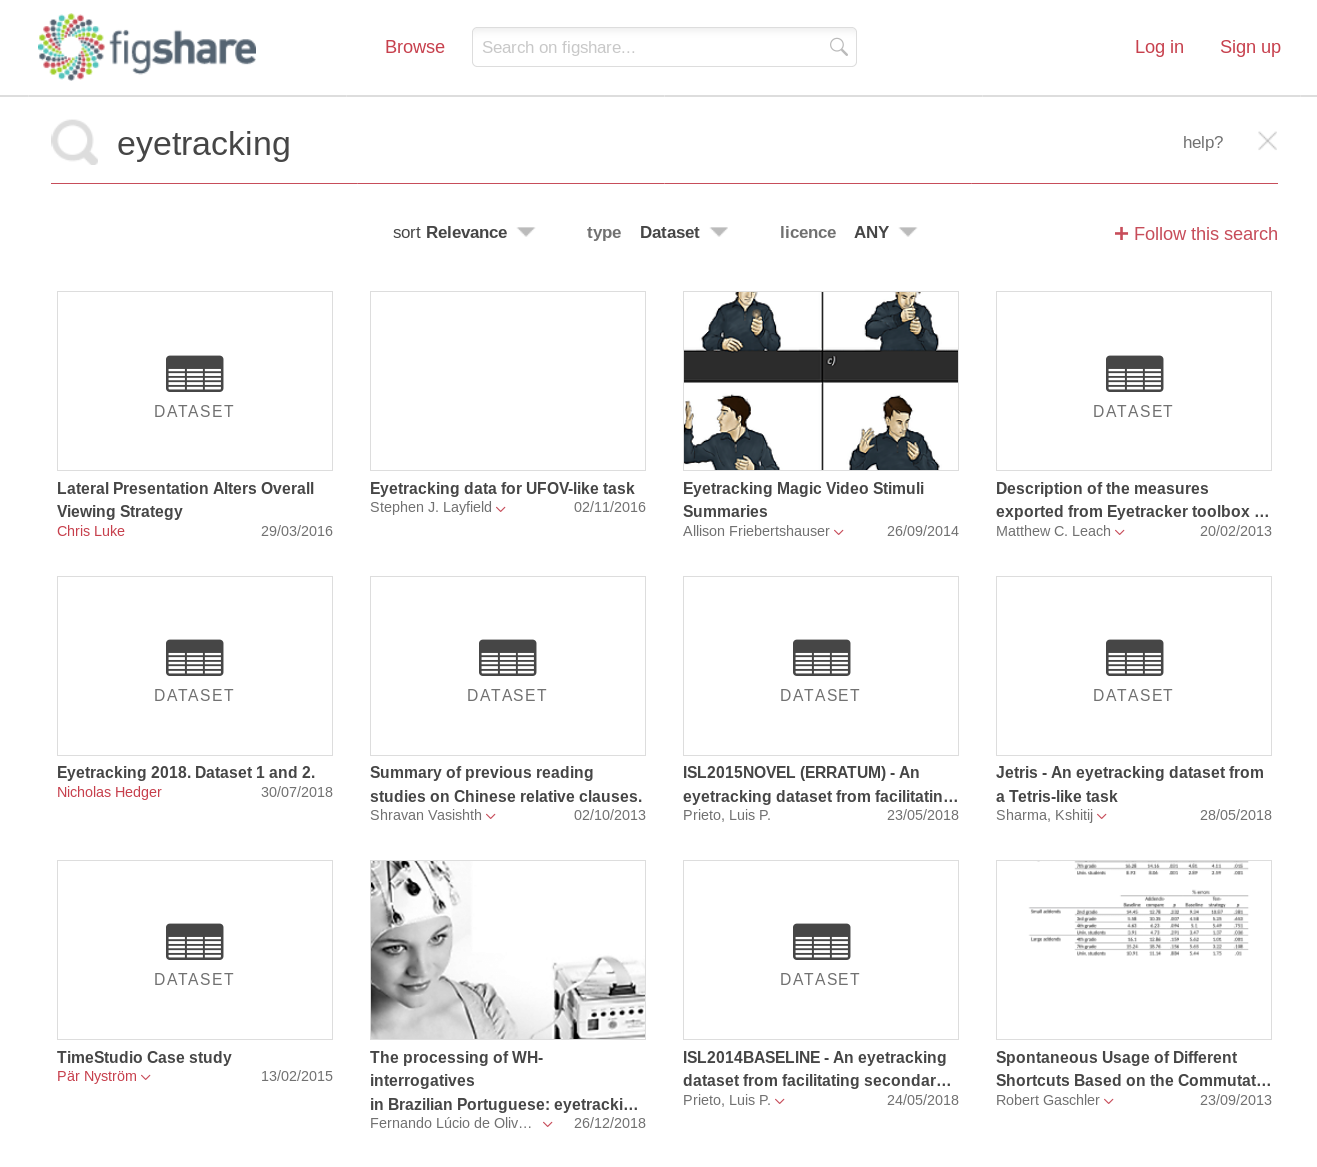
\includegraphics[height=\textheight]{figshare.png}
}

\frame{
\frametitle{Trolling}
   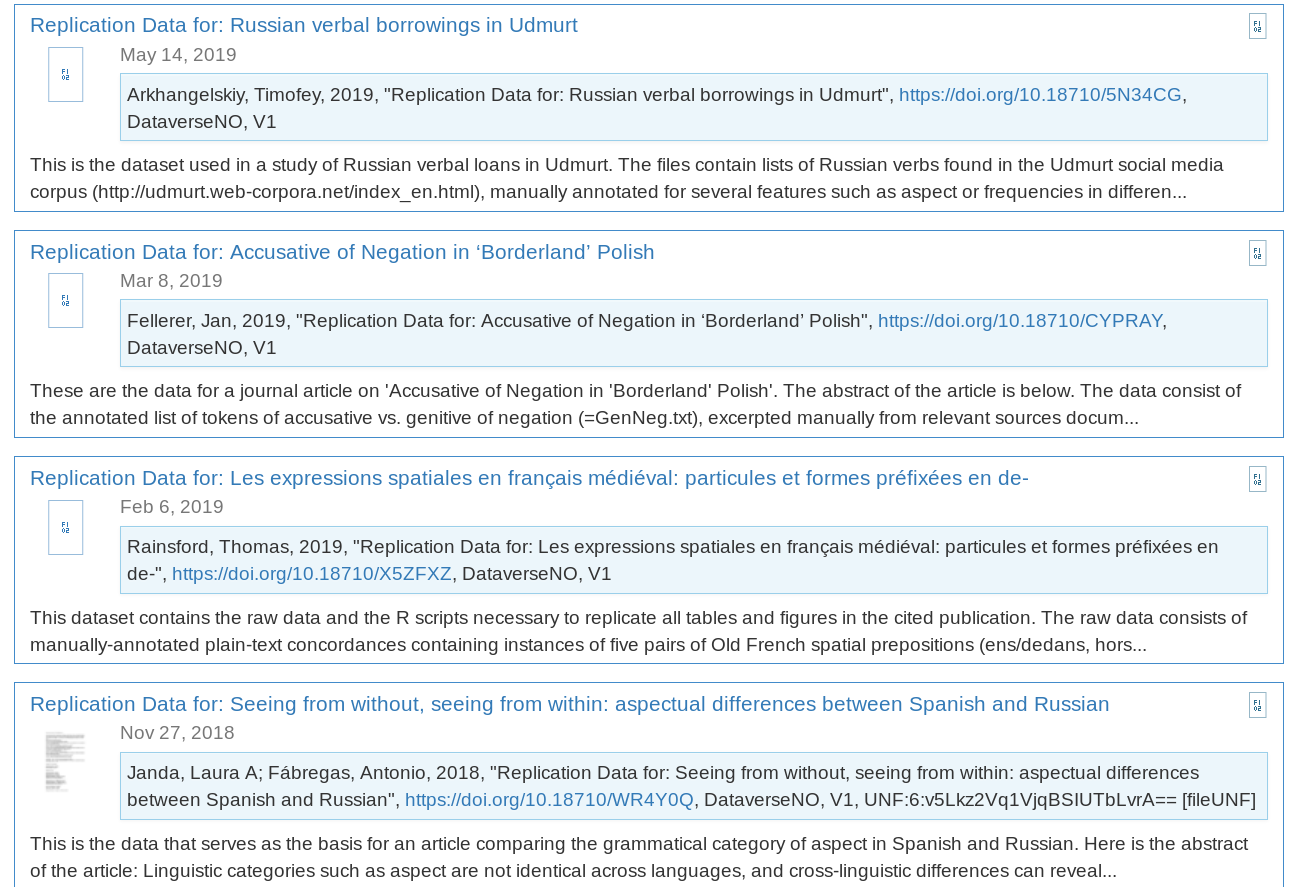
\includegraphics[height=\textheight]{trolling.png}
}


\frame{
\frametitle{Zenodo}
   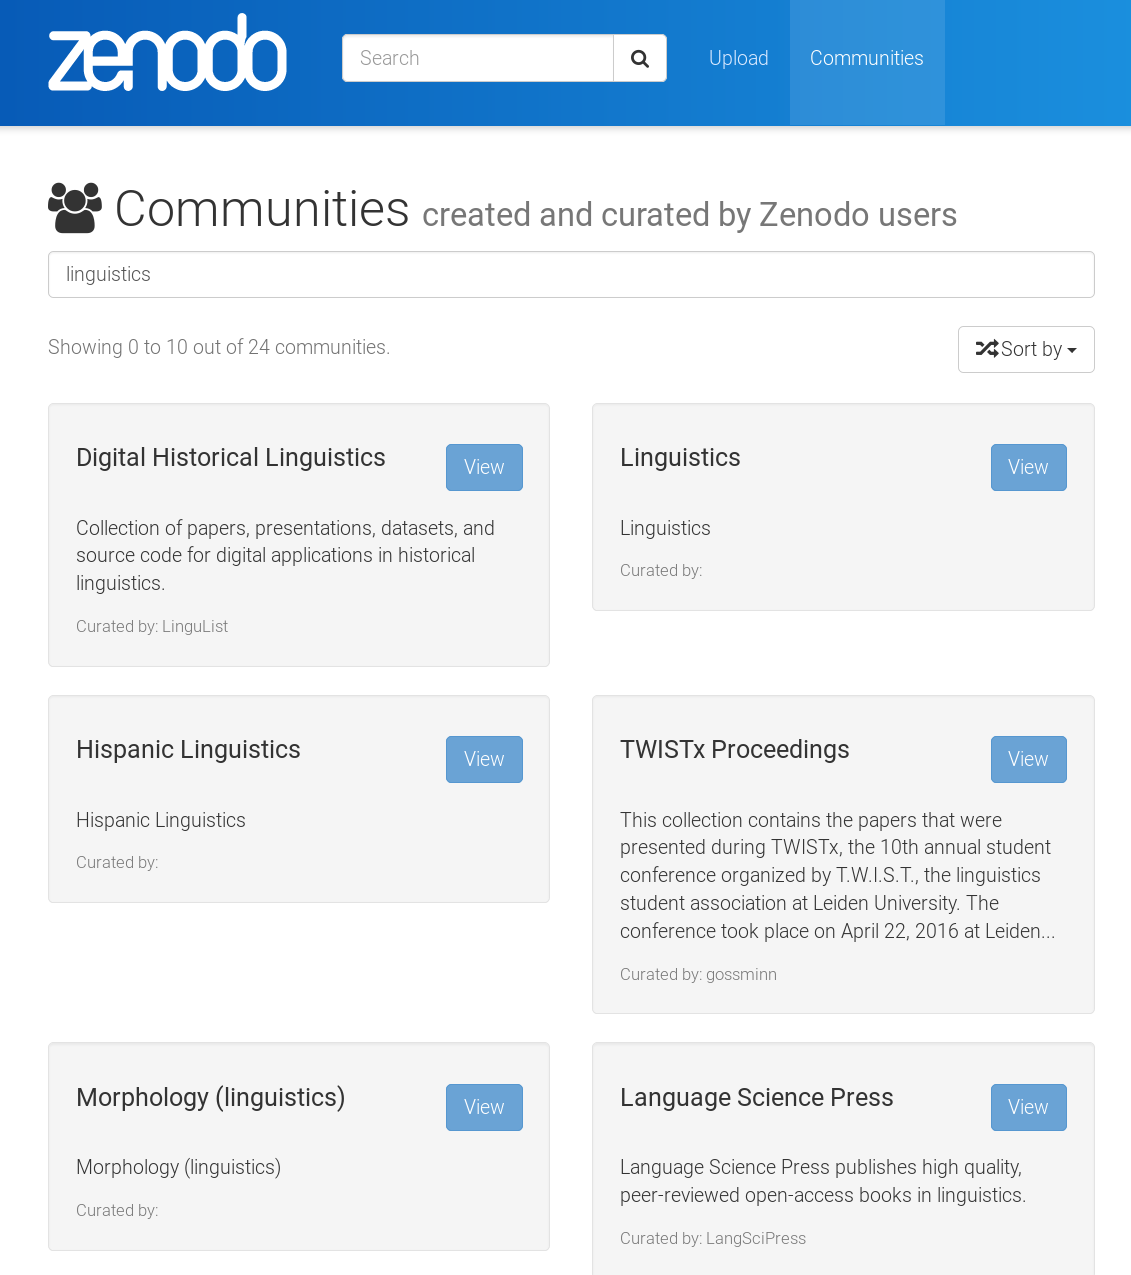
\includegraphics[height=\textheight]{zenodo.png}
}


\frame{
\frametitle{Repositories for texts: Preprint servers}
%   \includegraphics[height=.2\textheight]{./path/to/graphicsfile}
  \begin{itemize}
    \item
    \item
  \end{itemize}
}
\frame{
\frametitle{LingBuzz}
   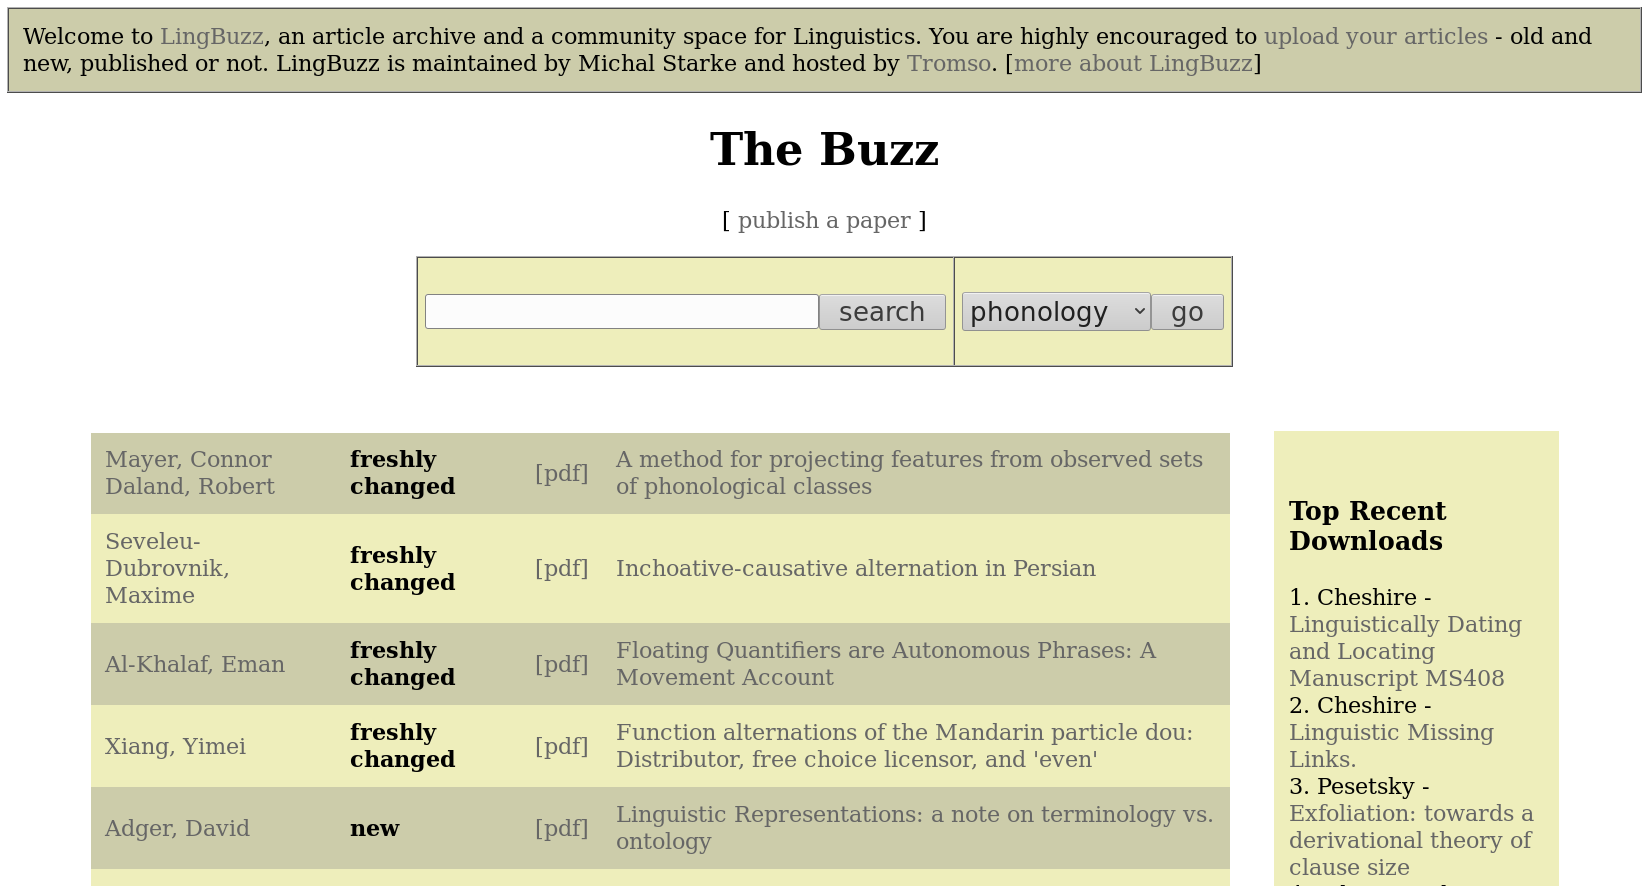
\includegraphics[height=\textheight]{lingbuzz.png}
}

\frame{
\frametitle{semanticsarchive.net}
   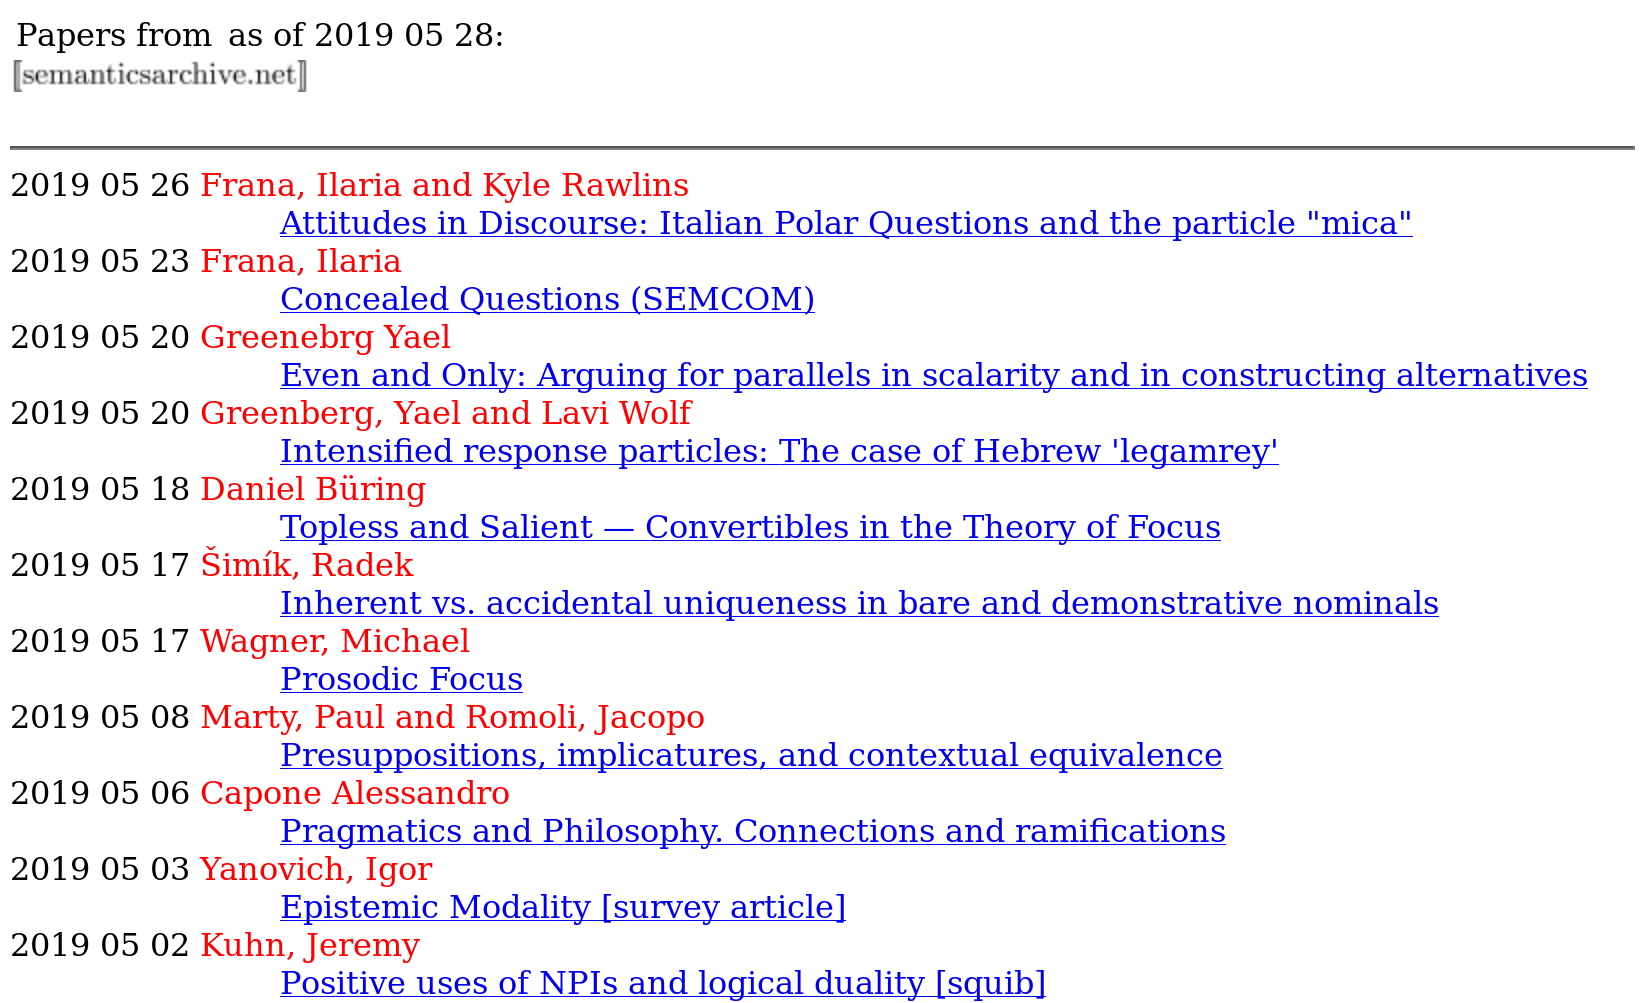
\includegraphics[height=\textheight]{semanticsarchive.png}
}

\frame{
\frametitle{Rutgers Optimality Archive}
   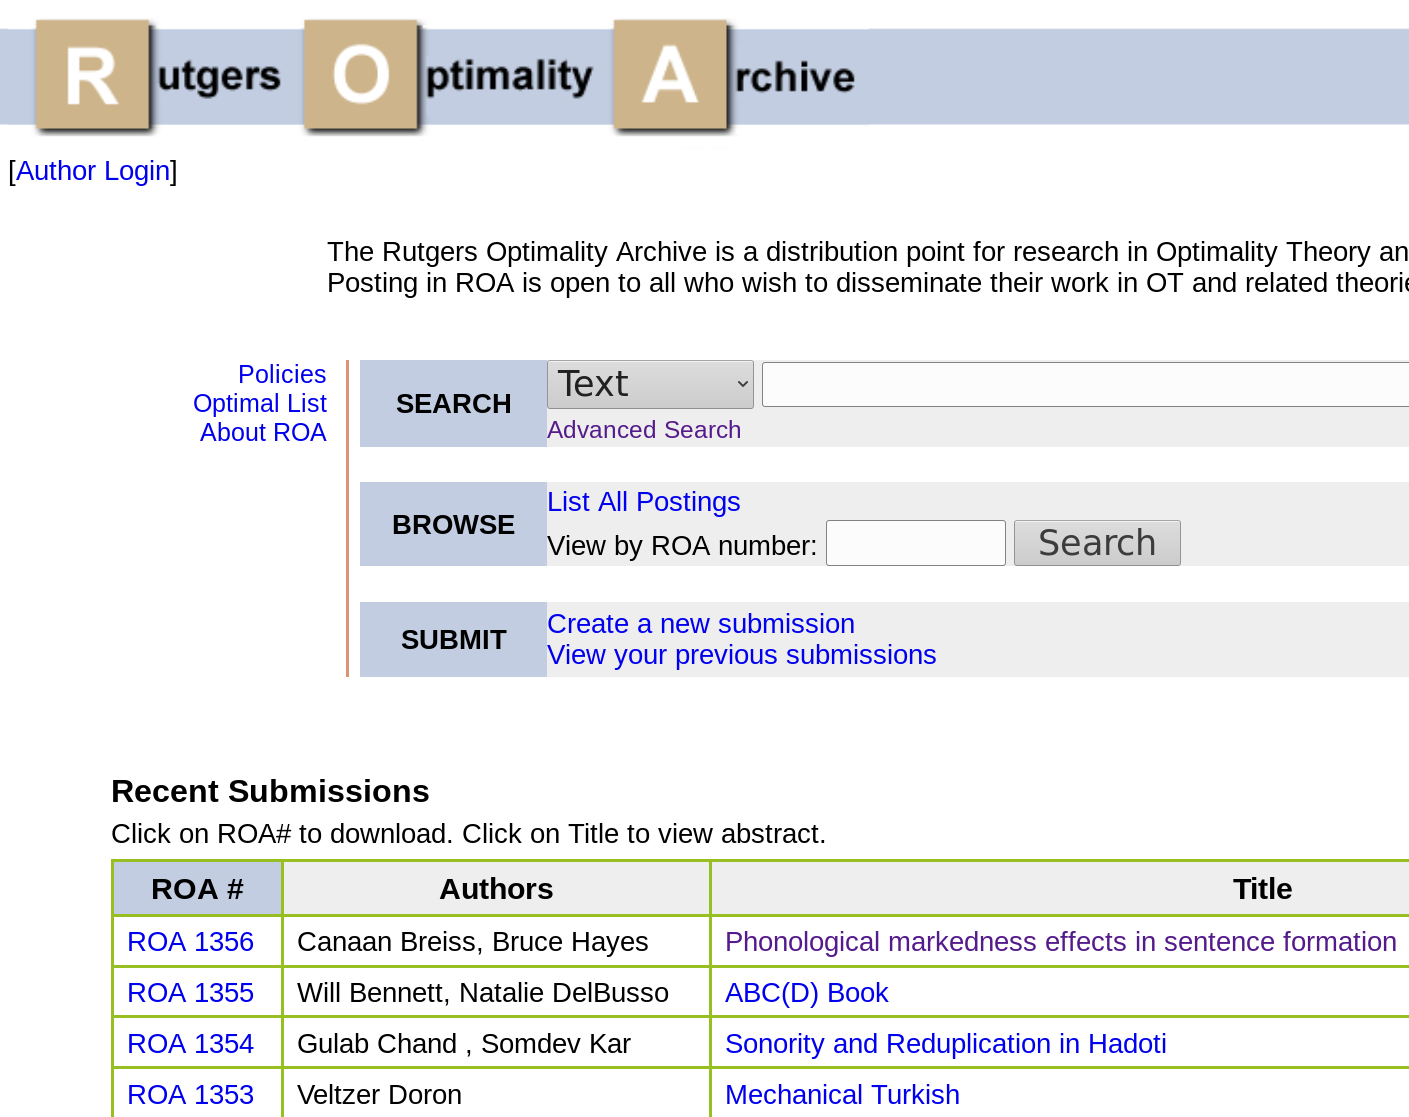
\includegraphics[height=\textheight]{roa.png}
}


\frame{
\frametitle{Academia and Researchgate}
  \begin{itemize}
    \item  Academia.edu and researchgate are NOT repositories
    \item both make money from \textbf{restricting} access
    \end{itemize}
}                    

\frame{
\frametitle{A note on scooping}
  \begin{itemize}
    \item  Scooping means that someone ``steals'' your research while you are still finalising it
    \item that fear is by and large unwarranted 
    \item you can count yourself happy if anybody IS actually interested in your data!
    \item most research actually struggles a lot more with a lack of interest to outsiders rather than scooping 
    \item preprint servers allow you to register your data and establish primacy
  \end{itemize}
}
            
\frame{
\frametitle{And now, finally: publications!}
%   \includegraphics[height=.2\textheight]{./path/to/graphicsfile}
  \begin{itemize}
    \item  raw data + code + write-up = publication
    \item journals
    \item books
    \begin{itemize}
      \item book chapters
    \end{itemize}

  \end{itemize}
}
            

\frame{
\frametitle{Intellectual Property Rights}
%   \includegraphics[height=.2\textheight]{./path/to/graphicsfile}
  \begin{itemize}
    \item  ``Copyright'' in the Anglo-Saxon countries
    \item  ``Urheberrecht/droit d'auteur'' in continental Europe
    \item These are different!
    \item Once you create something, you can decide who can use it and how
    \item Choose wisely and be explicit!
  \end{itemize}
}

\frame{
\frametitle{License}
%   \includegraphics[height=.2\textheight]{./path/to/graphicsfile}
  \begin{itemize}
    \item  Usage rights can be differentiated as follows
    \begin{itemize}
      \item geographical restriction (e.g. \textit{only for France})
      \item type restrictions (e.g. \textit{only for print}) 
      \item exclusive (no-one else has the right) vs. non-exclusive (other people may also get the rights)
      \item copyright transfer agreement (Anglo-Saxon culture)
      \item total buy-out
    \end{itemize}
  \end{itemize}
}

\frame{
\frametitle{Copyright transfer agreement}
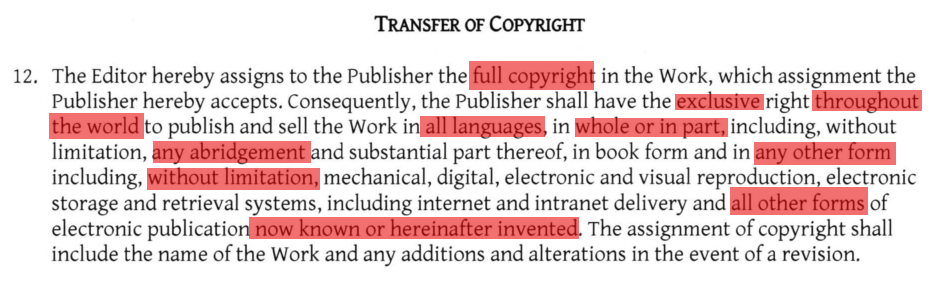
\includegraphics[width=\textwidth]{copyrighttransfer.pdf}
}

\frame{
\frametitle{Contracts}
%   \includegraphics[height=.2\textheight]{./path/to/graphicsfile}
  \begin{itemize}
    \item  Publisher contracts restrict everybody, including yourself 
    \item once you sign away your copyright, you have no longer the right to use your own material 
    \item to reuse tables or graphics in subsequent works of yours, you must first ask the new rights holder for permission 
    \item chasing rights is incredibly annoying
    \item publishers will put your content behind a paywall, meaning that it can actually be more difficult to access once it is officially published than before
    \item publisher vary as to whether and when they allow books to be hosted in repositories  
  \end{itemize}
    }

\frame{
\frametitle{Availability of Nordhoff (ed.) (2012)}
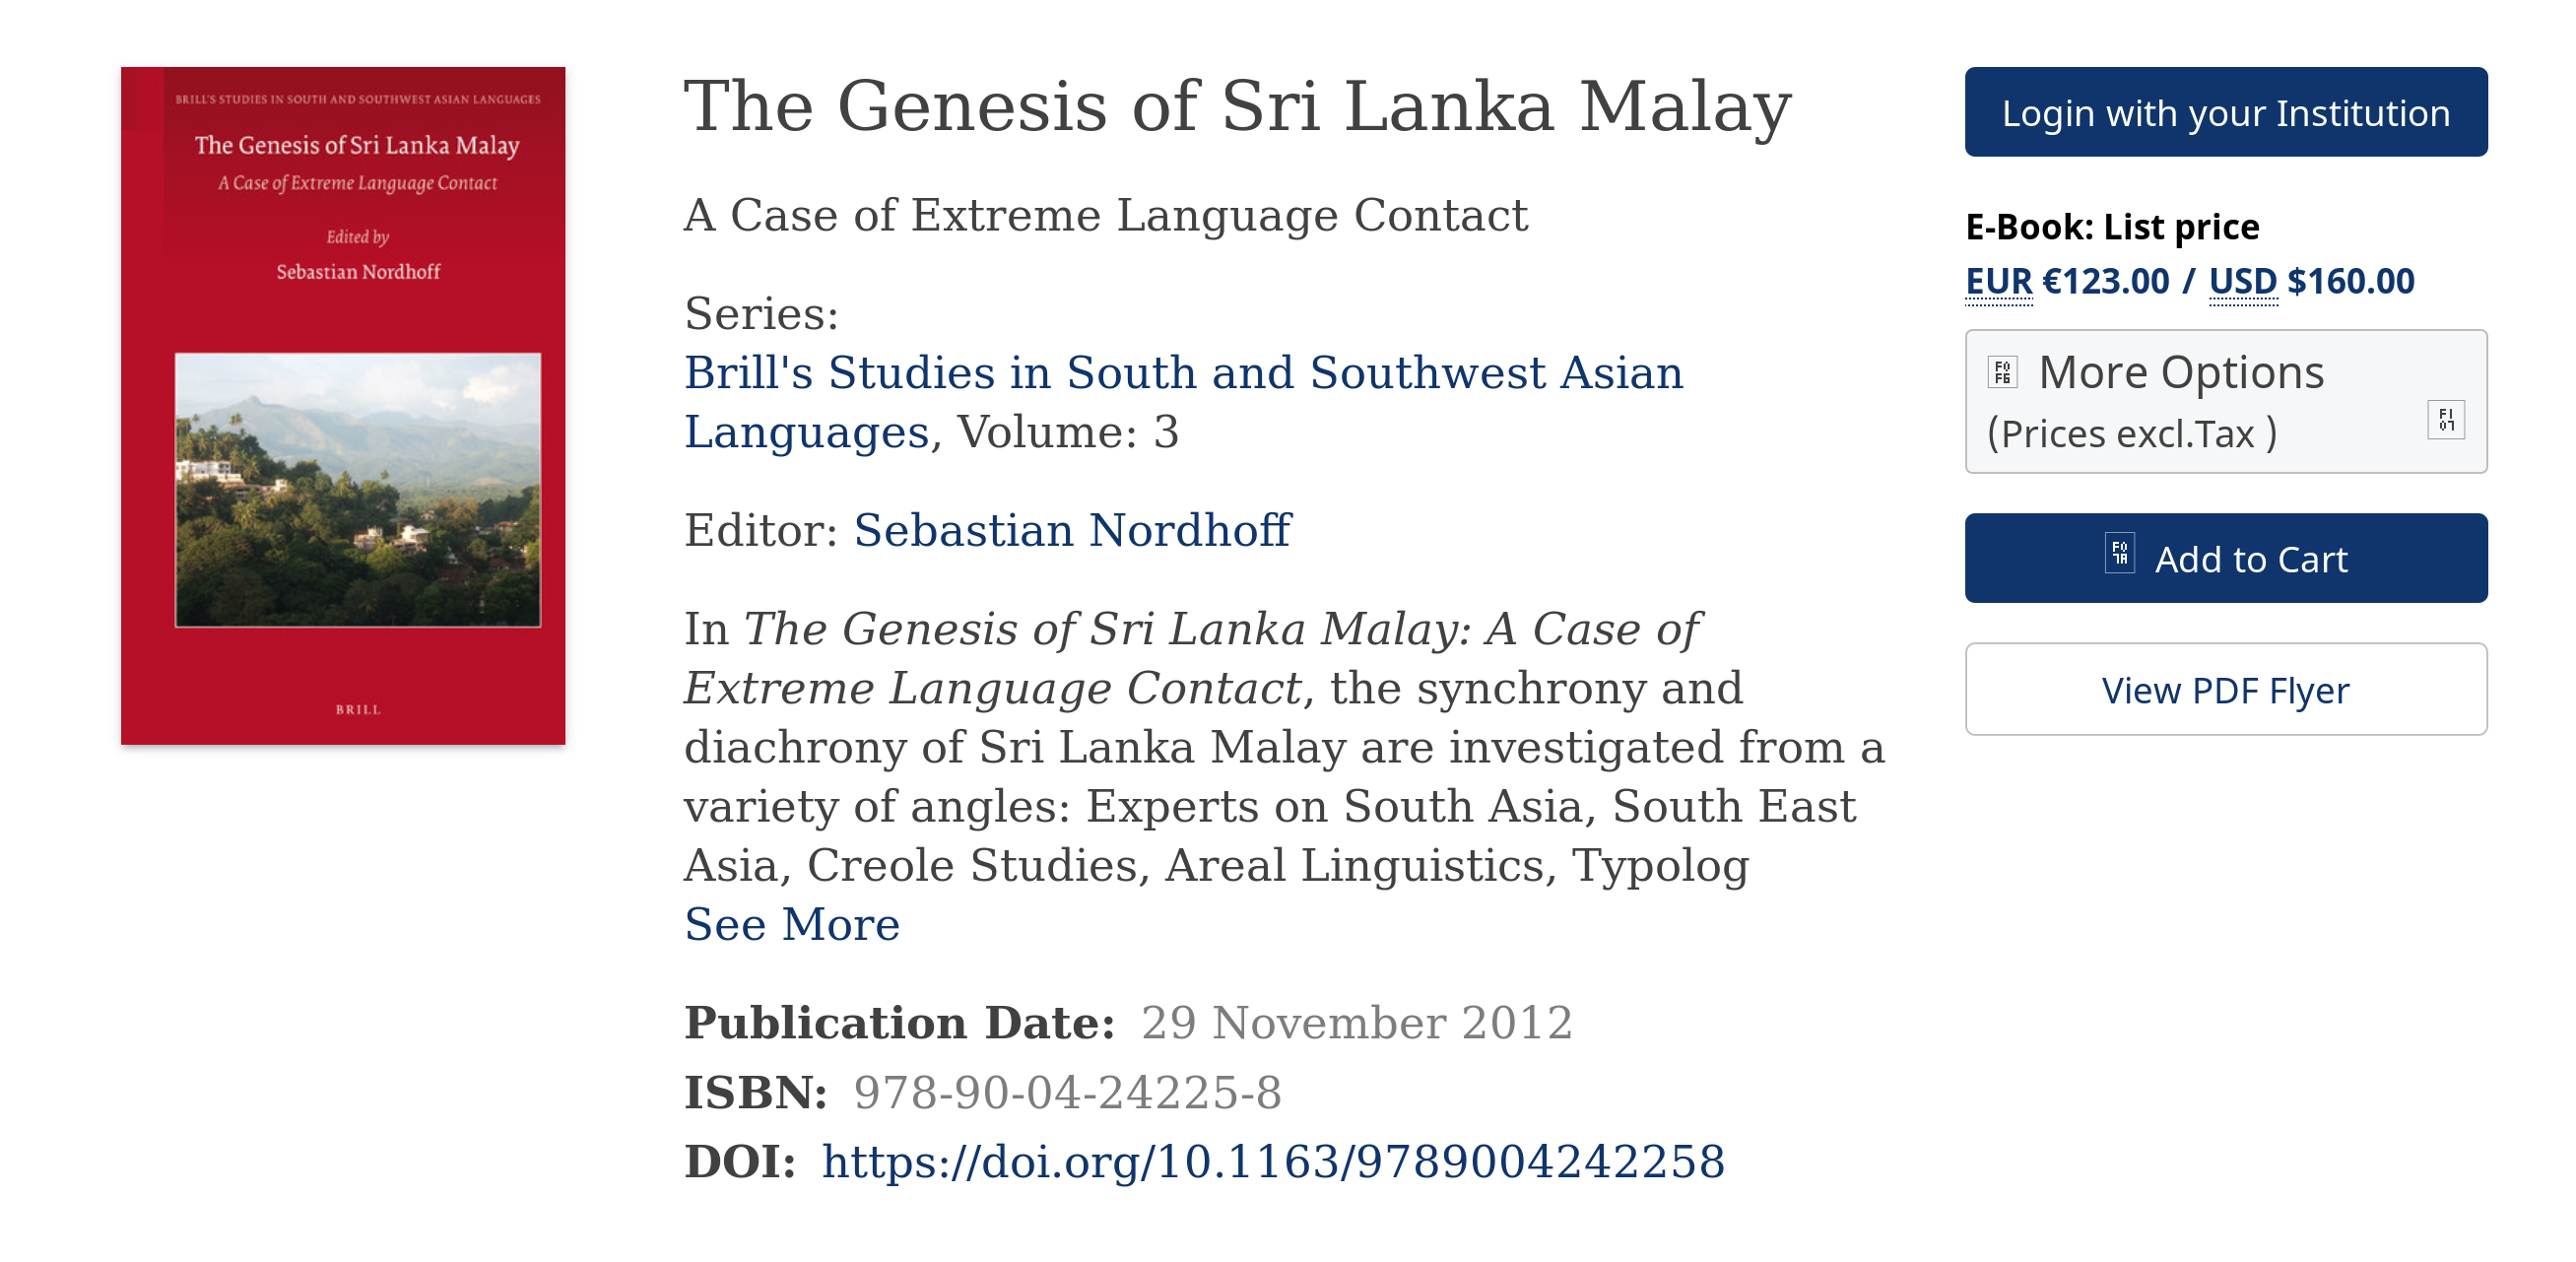
\includegraphics[width=\textwidth]{brillnordhoff.png}
 }

\frame{
\frametitle{Open Access colour codes}
%   \includegraphics[height=.2\textheight]{./path/to/graphicsfile}
  \begin{itemize}
    \item green
    \begin{itemize}
      \item Normal copyrighted publication with a publisher, but copy is archived in an institutional repository
    \end{itemize}
    \item gold
    \begin{itemize}
      \item publication is made openly available against a fee (Article Processing Charge, Book Processing Charge)
    \end{itemize}
    \item diamond
    \begin{itemize}
      \item like Gold OA, but without a fee
    \end{itemize}
      \item (black)
    \begin{itemize}
      \item a copyrighted publication is available via pirate sites/shadow libraries like SciHub or LibGen
    \end{itemize}
    \item (bronze)
    \begin{itemize}
      \item fake open access, not respecting the Berlin Declaration
    \end{itemize}
  \end{itemize}
}

\frame{
\frametitle{Articles}
%   \includegraphics[height=.2\textheight]{./path/to/graphicsfile}
  \begin{itemize}
    \item  FAIR open access principles
    <https://www.fairopenaccess.org/the-fair-open-access-principles/>
    \begin{itemize}
      \item The journal has a transparent ownership structure, and is controlled by and responsive to the scholarly community.
      \item Authors of articles in the journal retain copyright.
      \item All articles are published open access and an explicit open access licence is used.
      \item Submission and publication is not conditional in any way on the payment of a fee from the author or their employing institution, or on membership of an institution or society.
      \item Any fees paid on behalf of the journal to publishers are low, transparent, and in proportion to the work carried out.
    \end{itemize}
    \item Directory of Open Access Journals
    \item oaling.wordpress.com
  \end{itemize}
}

\frame{
\frametitle{Directory of Open Access Books (DOAB)}
%   \includegraphics[height=.2\textheight]{./path/to/graphicsfile}
  \begin{itemize}
    \item  \url{https://directory.doabooks.org/browse?type=classification_text&value=linguistics}
    \item
  \end{itemize}
}



\frame{
\frametitle{Thank you}
  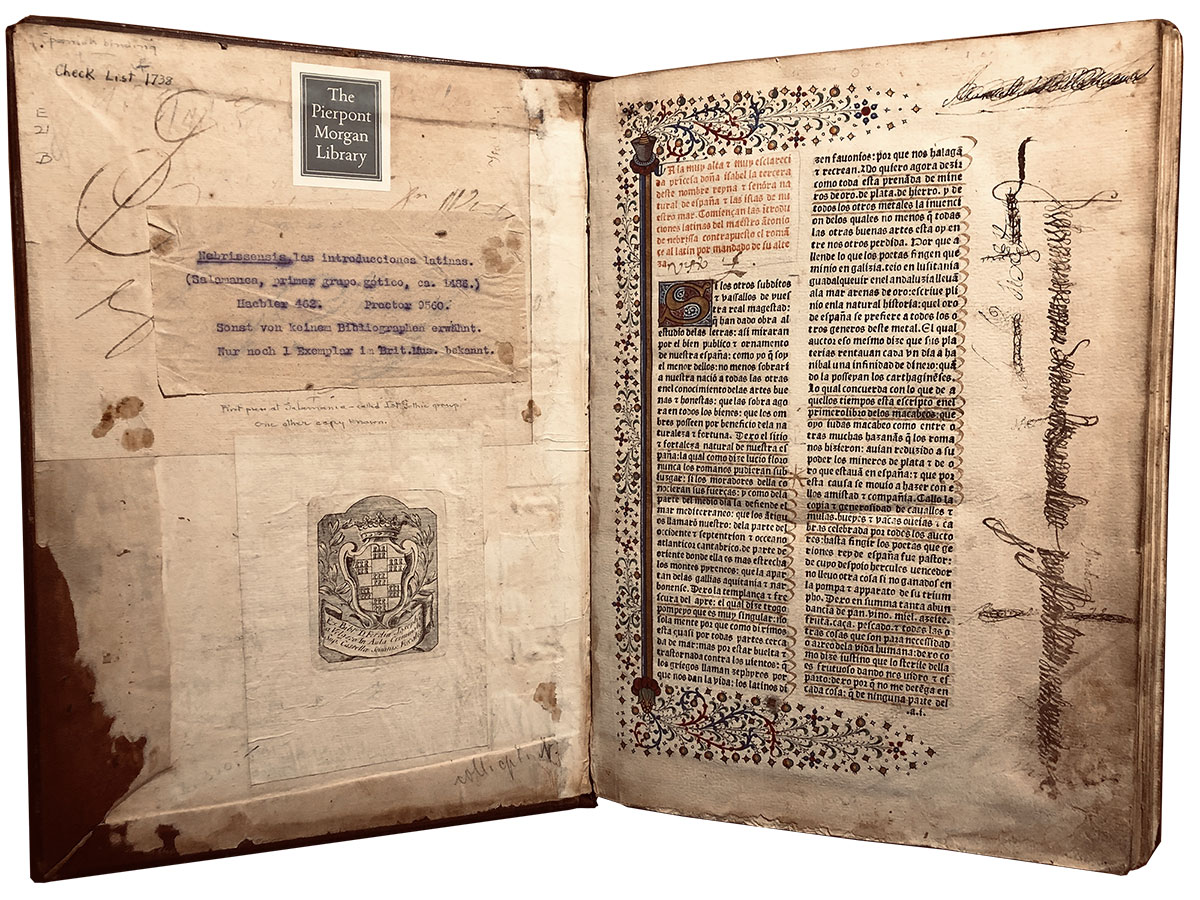
\includegraphics[width=\textwidth]{nebrija.jpg}
}    

\end{document}
